\documentclass[11pt]{article}

\usepackage[utf8]{inputenc}
\usepackage[T1]{fontenc}
\usepackage[margin=1in]{geometry}
\usepackage{amsmath,amssymb}
\usepackage{graphicx}
\usepackage{booktabs}
\usepackage{array}
\usepackage{caption}
\usepackage{enumitem}
\usepackage{microtype}
\usepackage{tikz}
\usetikzlibrary{arrows.meta,positioning,calc,fit,backgrounds,shapes.geometric}
\usepackage[hidelinks]{hyperref}
\usepackage{url}

\newcommand{\code}[1]{\texttt{#1}}

\tikzset{
  proc/.style={rectangle, rounded corners=3pt, draw=black!55, line width=0.7pt,
    fill=blue!5, align=center, inner sep=6pt, text width=6.4cm, font=\small},
  keynode/.style={proc, fill=black!6},
  certnode/.style={proc, fill=black!3, draw=black!70, line width=0.9pt},
  annot/.style={font=\footnotesize\itshape, text=black!55, align=left},
  flow/.style={-{Stealth[length=2.6mm]}, line width=0.8pt, draw=black!65},
  fb/.style={-{Stealth[length=2.6mm]}, line width=0.7pt, draw=black!45, dashed},
}

\title{\textbf{LLM-Assisted Trading Strategy Search:\\
Validation and the Limits of Automated Alpha Discovery}}

\author{Vincent Maciejewski\\
\small Independent Researcher\\
\small \texttt{mayeski@gmail.com}}

\date{\today}

\begin{document}
\maketitle

\begin{abstract}
Large language models (LLMs) write trading-strategy code fluently, yet they cannot tell whether a
strategy captures a real market effect or a pattern that only looks good in historical data. We
present LLM-Assisted Trading Strategy Search (LATSS), a FunSearch-style evolutionary loop in which an
LLM serves as a mutation operator over strategy structure while deterministic components fit
parameters by differential evolution and certify the result against a capacity-based skill bar
(the null-max bar), scored by cross-validated active Sharpe. The paper makes two contributions.
First, we validate the loop as a measurement instrument on a Magnificent-7 test-bed with synthetic
features of known signal strength. Mechanical (non-LLM) searchers that reuse the same evaluation
stack give high replication at no token cost, which lets us map a certification power curve over 30
seeds per point. Pure noise never certifies (0 of 30 runs; 95\% upper bound 11.6\%), and injected
signal is recovered and certified once its oracle active Sharpe passes roughly 0.66. We find that the bar's
false-positive rate is preserved, in part by construction, as the search budget grows to ten thousand
candidates on a high-capacity but finite class: capacity raises the bar rather than creating false
certifications. We also show that a bar computed over a
class smaller than the search is invalid, certifying pure noise in two of every three runs, and that
an LLM-driven search recovers signal at the same threshold as mechanical search. Second, we examine
the ceiling of the approach. LATSS, like other LLM alpha-mining systems, searches within a
human-supplied hypothesis space rather than performing the abductive step that creates a new one. We
formalize the distinction and show that withholding the predictive feature from the vocabulary drives
recovery to zero at every signal strength, independent of search effort. Code and experiments are
open source.
\end{abstract}

\section{Introduction}

An LLM can produce a valid, plausible-looking trading strategy on demand. What it cannot do is tell
whether the strategy works. It has no reliable way to separate a real market effect from an artifact
of the history it was fit to, and it has no cheap oracle to check its own output against, unlike a
chess engine with an authoritative board or a theorem prover that verifies a proof. The output is
fluent and confident with no built-in tie to the truth.

LATSS addresses this with a division of labor. The LLM is used as a search operator: it proposes and
mutates the structure of a candidate strategy. Deterministic components handle the two things the
model cannot do reliably. A numerical optimizer fits the free parameters, and an evaluator decides
whether a fitted candidate survives, using cross-validation and a skill bar. The design follows
FunSearch~\cite{funsearch}, where an LLM proposes programs, a systematic evaluator scores them, and
the best feed back into the next prompt. LATSS adapts the pattern to trading, whose scoring landscape
is far noisier and easier to overfit than FunSearch's exact-score problems.

Because the LLM can only combine the features it is given, the feature vocabulary defines the
discoverable strategy space. This paper separates two questions.

\begin{enumerate}[leftmargin=1.4em]
\item \textbf{Is the loop a sound instrument?} Given a feature that genuinely predicts, does the
search recover and certify it, and does certification reject noise? We answer this empirically
(Sections~\ref{sec:framework}--\ref{sec:results}) with synthetic controls of known signal strength.
A central move is to use mechanical (non-LLM) searchers that reuse the exact evaluation stack. They
cost no tokens, so we can replicate thirty to ten thousand times and treat the loop as an object of
measurement. The certification machinery, a purged and embargoed cross-validation and a
capacity-based null-max bar, is set out and compared with its alternatives in
Section~\ref{sec:method}.
\item \textbf{Can the loop invent new alpha?} We argue it cannot, as a property of the approach
rather than of any one implementation (Section~\ref{sec:ceiling}). LATSS searches a supplied
hypothesis space; it does not perform the abductive step that creates a new one.
\end{enumerate}

The two results pair together. An LLM-driven search can be turned into a trustworthy instrument for
signal that a human proposes, which is the role our experiments support.

\paragraph{Contributions.} (i) A controlled benchmark for LLM strategy-search systems, with synthetic
features of known signal strength and mechanical searchers that reuse the same evaluation stack. (ii)
A same-class empirical null-max certification procedure, and a demonstration that a bar computed over a
class smaller than the search is invalid. (iii) A capacity experiment showing the certification
threshold rises with search budget while the calibrated certification frequency on noise stays
controlled. (iv) A vocabulary-boundary test showing that search does not recover signal excluded from
its representation. We do not claim that LATSS discovers a profitable trading strategy.

\section{Related work}
\label{sec:related}

\paragraph{Program search with LLMs.} FunSearch~\cite{funsearch} established the
propose--score--feedback loop with an LLM as mutation operator, finding new cap-set constructions and
improved bin-packing heuristics. Later systems generalize the pattern. The common structure is an
evolutionary search over programs in which the LLM supplies variation and a deterministic evaluator
supplies selection.

\paragraph{LLM alpha mining.} A growing family applies this loop to finance, searching formulaic
factors over raw price and volume with a fixed operator language: AlphaAgent~\cite{alphaagent},
``Automate Strategy Finding with LLM''~\cite{automate}, CogAlpha~\cite{cogalpha},
Hubble~\cite{hubble}, QuantaAlpha~\cite{quantaalpha}, AlphaLogics~\cite{alphalogics},
EFS~\cite{efs}, and reinforcement-learning miners such as AlphaGen, surveyed
in~\cite{evolutionalpha}. These differ from LATSS in scope, searching factor formulas over raw
inputs rather than strategies over given indicators, and in machinery, with multi-agent hierarchies,
tree search, sandboxes, and novelty regularizers. They share one paradigm: recombination of a
human-defined primitive vocabulary. Section~\ref{sec:ceiling} returns to what this line does and does
not solve.

\paragraph{Overfitting and evaluation.} Certification here rests on capacity-based reasoning about
how much apparent skill luck can produce: VC-style bounds~\cite{vapnik}, empirical Rademacher
complexity~\cite{bartlett}, purged and embargoed cross-validation and the Deflated Sharpe
Ratio~\cite{deprado,deflated}, and the null-max construction~\cite{nullmax}. We use an empirical
null-max (Rademacher) bar as the operative gate for the reasons in Section~\ref{sec:bar}.

\section{The LATSS framework}
\label{sec:framework}

LATSS searches for a trading strategy expressed as a function of features, the object a quantitative
analyst otherwise hand-designs. The architecture is not tied to a particular market.

\begin{enumerate}[leftmargin=1.4em]
\item \textbf{Representation.} A candidate is a scoring function $\code{score}(\text{features}, p)$
mapping features to a trading decision, with numeric parameters $p$.
\item \textbf{Search.} A language model proposes and mutates the scoring function, acting as the
mutation operator. It never sees prices and never picks a numeric value; it sees the scored history
of previously proposed structures and emits a new structure. Differential evolution then fits $p$.
\item \textbf{Fitness.} Each candidate is backtested and scored by its cross-validated median
out-of-sample Sharpe against a benchmark, the passive alternative for the use case. For a universe
selector the benchmark is the equal-weight portfolio, so fitness is the active Sharpe of the strategy
over equal-weight. The loop keeps the highest-fitness candidate, the champion.
\item \textbf{Certification.} The champion is credited with skill only if its active Sharpe clears a
skill bar (Section~\ref{sec:bar}).
\end{enumerate}

\begin{figure}[htbp]
\centering
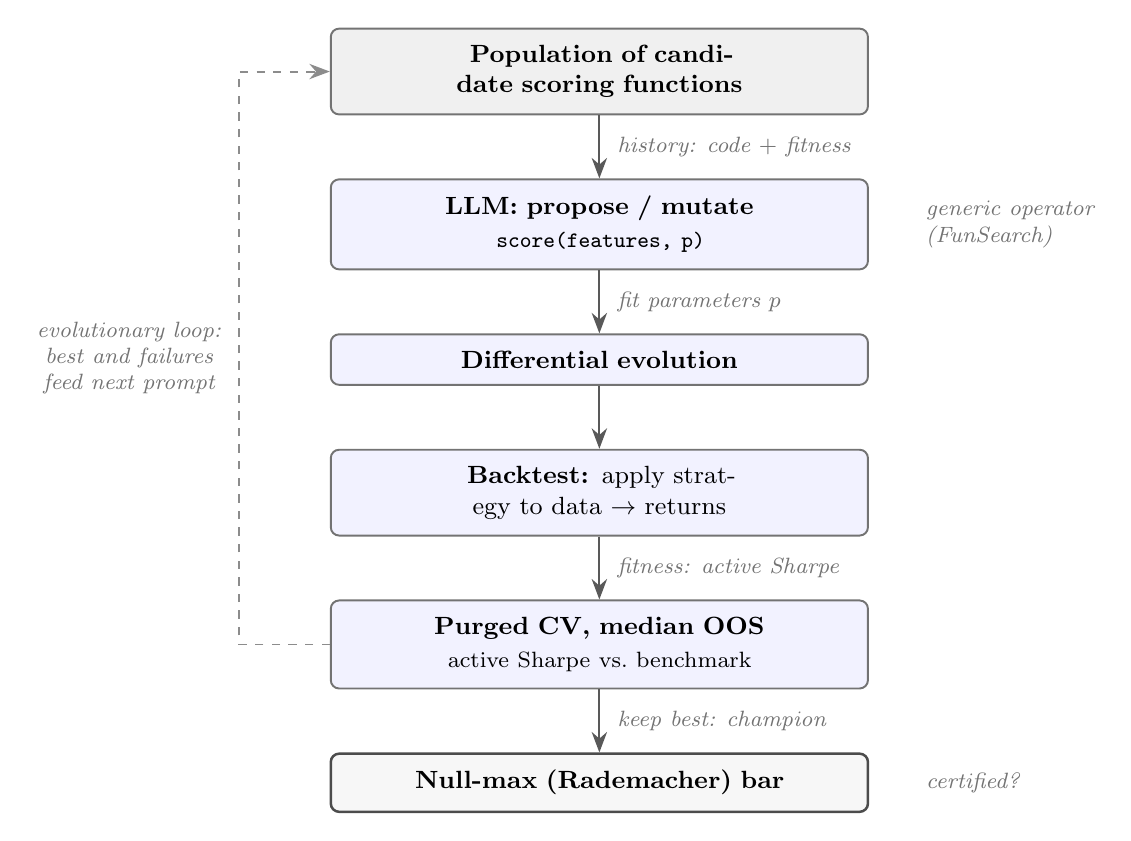
\begin{tikzpicture}[node distance=8mm and 6mm]
  \node[keynode] (pop) {\textbf{Population of candidate scoring functions}};
  \node[proc, below=of pop] (llm)
    {\textbf{LLM: propose / mutate}\\[1pt]{\ttfamily\footnotesize score(features, p)}};
  \node[proc, below=of llm] (de) {\textbf{Differential evolution}};
  \node[proc, below=of de] (bt)
    {\textbf{Backtest:} apply strategy to data $\rightarrow$ returns};
  \node[proc, below=of bt] (cv)
    {\textbf{Purged CV, median OOS}\\[1pt]{\footnotesize active Sharpe vs.\ benchmark}};
  \node[certnode, below=of cv] (bar) {\textbf{Null-max (Rademacher) bar}};
  \draw[flow] (pop) -- node[annot, right=1mm] {history: code $+$ fitness} (llm);
  \draw[flow] (llm) -- node[annot, right=1mm] {fit parameters $p$} (de);
  \draw[flow] (de)  -- (bt);
  \draw[flow] (bt)  -- node[annot, right=1mm] {fitness: active Sharpe} (cv);
  \draw[flow] (cv)  -- node[annot, right=1mm] {keep best: champion} (bar);
  \coordinate (l1) at ($(cv.west)+(-1.15,0)$);
  \coordinate (l2) at ($(pop.west)+(-1.15,0)$);
  \draw[fb] (cv.west) -- (l1) -- (l2)
    node[annot, midway, left=1mm, align=center] {evolutionary loop:\\ best and failures\\ feed next prompt} -- (pop.west);
  \node[annot, right=6mm of llm] {generic operator\\ (FunSearch)};
  \node[annot, right=6mm of bar] {certified?};
\end{tikzpicture}
\caption{The LATSS loop. The LLM proposes and mutates strategy structure from the scored history,
differential evolution fits parameters, and the evaluator scores by cross-validated active Sharpe and
certifies the champion against the null-max bar.}
\label{fig:loop}
\end{figure}

\subsection{Two use cases}

In the generative use, given candidate indicators, the loop searches for a scoring rule that combines
them, and a champion is trustworthy only if its cross-validated active Sharpe clears the bar. In the
diagnostic use, the candidate indicator is handed to the loop among null predictors with the identity
withheld; recovering and certifying it across seeds is evidence of real signal. Both uses need the
same instrument property: reject noise, and recover genuine signal of sufficient strength.

\section{Validation methodology}
\label{sec:method}

We validate the loop with controlled ground truth. The loop is instantiated on a concrete market with
the input features replaced by synthetic features of known signal content.

\paragraph{Test-bed.} The universe is the seven ``Magnificent-7'' US equities (AAPL, MSFT, GOOGL,
AMZN, NVDA, META, TSLA), daily from 2015 to 2026 (2{,}952 bars, about 11.7 years). The universe is
fixed in advance and the predictive features are synthetic, so survivorship and universe-selection
effects do not enter these experiments. Each bar the strategy holds the single highest-scoring name,
and the benchmark is the equal-weight portfolio. The
metric throughout is active Sharpe, the annualized Sharpe of the strategy's daily return over the
equal-weight benchmark, which isolates selection skill. A single name inherits the basket's
bull-market Sharpe, so a standalone Sharpe would overstate skill.

\paragraph{Synthetic features.} The selector is given four opaquely named per-name features,
\code{feat\_a} through \code{feat\_d}. In the negative control all four are persistent (AR(1),
$\phi=0.9$) unit-variance noise. In the positive control one hidden slot (\code{feat\_c}) is a
cross-sectional predictor: for every name $n$ and time $t$,
\begin{equation}
\code{feat\_c}[n,t] \;=\; \rho \, z[n,t] \;+\; \sqrt{1-\rho^{2}}\;\varepsilon[n,t],
\label{eq:synth}
\end{equation}
where $z[n,t]$ is a standardized forward excess return and $\varepsilon$ is unit-variance noise. With
a forward horizon $h=21$ trading days, the forward excess return is
$\mathrm{ex}[n,t]=p[n,t{+}h]/p[n,t]-1$ minus its cross-sectional mean across names at $t$, and
$z[n,t]$ standardizes $\mathrm{ex}$ per name over the full sample. The weight $\rho^{2}$ is the
fraction of \code{feat\_c}'s variance that is true signal, and $\sqrt{1-\rho^{2}}$ holds it at unit
variance so only its signal content changes with $\rho$. The searcher is told none of this.
\code{feat\_c} is a deliberate synthetic oracle built from future returns, used to set a known signal
strength; it is the predictor under test rather than a tradable feature, and is the only route by
which forward information enters the experiment.

\paragraph{Cross-validation.} We use purged, embargoed, chronological $k$-fold~\cite{deprado}. The
pool is cut into six contiguous blocks; each serves once as the test fold, and training is every
other bar except an embargo band of 250 trading days on each side of the test block. The embargo
exceeds the longest feature lookback, so no training bar shares a lookback window with a test bar. We
avoid the common alternative of random 75/25 quarter splits, in which adjacent quarters overlap
through warm-up and the split is not chronological. A permissive scheme is doubly damaging, because
fitness and the noise bar are computed under the same cross-validation, so leakage inflates a
signal's score and lowers the bar at the same time.

\paragraph{Searchers.} The LLM proposes structures through a subagent interface that needs no API key
(Section~\ref{sec:e7}). For high-replication measurement we also use three mechanical searchers over
the same scoring contract and evaluation stack: a bounded linear class with weights fit by
differential evolution; a high-capacity nonlinear class of random expression trees over the four
features, parameter-free so that a search budget of ten thousand candidates is cheap; and genetic
programming over the same grammar. The nonlinear class is the adversarial case for the bar among the
three, fitting noise far better than the linear class. It is a high-capacity proxy for an LLM emitting
arbitrary code, not that class itself: its random trees are finite-capacity, with finite VC dimension,
unlike the arbitrary-code case in Eq.~\eqref{eq:vc}.

\paragraph{Three notions of capacity.} We distinguish \emph{search capacity} (how expressive the
candidate class is), \emph{evaluation capacity} (how much parameter fitting happens inside each
candidate), and \emph{search budget} (how many candidates are evaluated). The mechanical nonlinear
class has a fixed search capacity and a tunable search budget, while the LLM code-writing case has a
much larger, effectively open search capacity. The capacity sweep (Section~\ref{sec:e4}) varies the
search budget alone.

\subsection{The null-max skill bar}
\label{sec:bar}

Under a sufficiently expressive, persistent search no partition of the data is truly out of sample
(Section~\ref{sec:ceiling}), so we do not certify against a hold-out. We certify in sample against a
null-max bar~\cite{nullmax}, the highest cross-validated active Sharpe the strategy class reaches on
data whose signal has been destroyed. A champion that cannot beat what its own class extracts from
noise has no measured skill.

\paragraph{Analytical bar (VC, worst case).} For a class of VC dimension $h$ over $m$ sessions
spanning $Y$ years, luck alone cannot exceed an annualized Sharpe of order
\begin{equation}
\mathrm{bar}_{\mathrm{VC}} \;\approx\; \sqrt{\tfrac{2\,h\,\log(e\,m/h)}{Y}} .
\label{eq:vc}
\end{equation}
This is a rough capacity scale rather than a bound derived for our exact procedure: the constant does
not fold in the argmax selection step or the dependence across observations. As an order of magnitude,
a linear combination of the four features ($h\approx 5$) sits near 2.5 at our sample size, while an
unconstrained code-writing class has effectively unbounded $h$ and no finite scale.

\paragraph{Empirical bar (Rademacher, operative).} The VC bar is adversarial, a ceiling rather than a
working hurdle. The operative bar is measured on the data. For each scramble we multiply every entry
of the $T\times N$ return matrix by an independent random sign, destroying any relation between
features and returns while preserving return magnitudes, then refit every candidate in the allowed
class under the same cross-validation and take the best-in-class median out-of-sample active Sharpe.
The distribution over scrambles gives the bar; we use its 95th percentile, written $\mathrm{bar}_q$.
The VC expression is a conservative capacity-based reference scale; the empirical null-max bar is the
operative calibration.

\paragraph{Same-class condition and certification.} The bar is valid only when the candidates refit
to noise span the same class the search may emit. A bar computed over a smaller class underestimates
the achievable noise fit and admits overfits, which Section~\ref{sec:ablation} measures. A champion
is credited with skill when its cross-validated active Sharpe exceeds $\mathrm{bar}_q$; we also report
the margin $\eta=\mathrm{CV}^{2}/\mathrm{bar}_q^{2}$, where $\eta\ge 2.5$ marks a comfortable clear.
The VC bar is reported as a ceiling and is never used as the gate. Certification means only that the
observed champion exceeds the empirical 95th-percentile null maximum under the stated class, search
procedure, and null construction. It is not a guarantee of future profitability.

\subsection{Null construction and its assumptions}
\label{sec:nullassume}

The sign flip multiplies each entry of the return matrix by an independent $\pm 1$. This removes the
feature-to-return relation, and with it the temporal dependence, the cross-sectional and common-factor
structure, and the volatility-state relationships present in the real panel. The bar is therefore the
best in-class fit under a null in which returns are independently sign-randomized conditional on their
magnitudes. It is a valid reference for this selector under a directional-signal assumption: absent a
feature-to-return relation, the sign of each name's return is exchangeable at the resolution the
selector acts on, and the long-only top-one selection earns the held name's return, whose sign the
flip removes. The bar's operating characteristics under richer dependence structures are not
established here. Nulls that preserve more structure, a by-day sign flip, a cross-sectional permutation of
returns across names, and block or stationary bootstraps, would test robustness to that assumption,
and we leave them to future work.

\subsection{Alternatives to the null-max bar}
\label{sec:whybar}

The standard alternatives are each unsuited to this setting. The Deflated Sharpe
Ratio~\cite{deflated} deflates by a trial count, but for an automated search the trial count is
ill-defined, since the search effectively covers the whole class, and it is gameable because fewer
trials incur a smaller penalty. The invariant that matters is the class's capacity, which the
null-max bar measures. Permutation and shift-the-signal tests select by a uniform maximum over
sampled configurations, while the fitness selects by differential evolution, which digs deeper into
noise, so they under-price the overfitting that produced the champion; we keep shift-the-signal only
as a reported diagnostic. A hold-out is not automatically sufficient when it becomes part of an
iterative research loop: with an expressive class and repeated adaptive re-use of the reserved period
across attempts, the hold-out is fit too. A genuinely untouched hold-out, used once at the end, does
give protection; the concern here is the iterative case.

\section{Experiments and results}
\label{sec:results}

All runs use purged, embargoed cross-validation and the empirical null-max bar. ``Clears'' means the
champion's cross-validated active Sharpe exceeds the bar. Mechanical conditions use at least 30
independent seeds; the LLM condition uses 3 seeds per point. The scripts producing every table are in
the repository.

\subsection{The null-max bar (E3)}
\label{sec:e3}

Over 1000 sign-flip scrambles, the 95th-percentile bar is $+0.844$ for the high-capacity nonlinear
class and $+0.408$ for the bounded linear class. The gap reflects both capacity and search mechanism:
the linear class is fit by continuous differential evolution and the nonlinear class by discrete
enumeration of trees, so the two are not a controlled capacity comparison. The classes also differ in
how fast the estimate settles. The nonlinear bar is stable beyond roughly 100 scrambles; the linear
bar keeps rising as scrambles increase, with a growing tail maximum, so a small scramble count
under-estimates a low-capacity bar. Experiments E1, E5, E7, and E12a use the 1000-scramble bar; the
capacity sweep (Section~\ref{sec:e4}) recomputes the bar at 100 scrambles per budget over the
nonlinear class, which the stability result shows is adequate.

\subsection{Power curve and false positives (E1)}
\label{sec:e1}

Table~\ref{tab:power} gives the certification rate against injected signal, 30 seeds per point, each
class certified against its own bar.

\begin{table}[htbp]
\centering
\caption{Certification power curve (30 seeds per point). ``Oracle'' is the active Sharpe a perfect
selector on \code{feat\_c} attains at that $\rho$, a descriptive full-sample quantity used only to set
signal strength and never seen by the search or certification. The certification frequency on noise
($\rho=0$) is 0 of 30 for both classes.}
\label{tab:power}
\small
\begin{tabular}{c c c c c}
\toprule
$\rho$ & oracle Sharpe & nonlinear $P(\text{clear})$ & median champ & linear $P(\text{clear})$ \\
\midrule
0.00 & $-0.67$ & 0.00 & $+0.44$ & 0.00 \\
0.10 & $\phantom{+}0.00$ & 0.03 & $+0.68$ & 0.00 \\
0.15 & $+0.30$ & 0.43 & $+0.83$ & 0.10 \\
0.20 & $+0.66$ & 1.00 & $+1.10$ & 0.70 \\
0.25 & $+0.95$ & 1.00 & $+1.40$ & 0.80 \\
0.30 & $+1.23$ & 1.00 & $+1.77$ & 1.00 \\
0.40 & $+1.66$ & 1.00 & $+1.96$ & 1.00 \\
0.50 & $+2.06$ & 1.00 & $+2.17$ & 1.00 \\
0.70 & $+2.81$ & 1.00 & $+2.79$ & 1.00 \\
\bottomrule
\end{tabular}
\end{table}

The boundary is sharp. Nothing clears at an oracle Sharpe at or below zero, and clearing becomes
reliable for the nonlinear class from $\rho=0.20$, where the oracle Sharpe is about 0.66; the linear
class reaches reliable clearing at $\rho=0.30$. The observed certification frequency on noise
($\rho=0$) is 0 of 30, a 95\% Clopper-Pearson upper bound of 11.6\%; rates below are observed
frequencies across seeds, not asymptotic probabilities. Constraining the class to linear does not buy sensitivity here: the nonlinear
class certifies at $\rho=0.20$ and $0.25$ more reliably than the linear class, because its champion
overfits above its higher bar while the linear champion grazes its lower bar with more seed-to-seed
variance. The two classes carry different bars, and neither dominates on detection power.

\subsection{Search amplification (E2)}
\label{sec:e2}

The champion's cross-validated score routinely exceeds the oracle ceiling. At $\rho=0.20$ the oracle
is 0.66 while nonlinear champions reach about 1.10, because the loop fits noise features on top of the
real signal. The amplification is why the operative hurdle is the bar near 0.6 to 0.8 and not the
oracle ceiling: the champion must beat what a same-capacity class extracts from noise, which it does
once real signal is present.

\subsection{Same-class ablation (E5)}
\label{sec:ablation}

We certify nonlinear champions against the correct nonlinear bar ($0.844$) and against a mismatched
linear bar ($0.408$), a class smaller than the search. On pure noise the correct bar certifies in 0 of
30 runs (95\% upper bound 11.6\%), while the mismatched bar certifies in 20 of 30 (95\% interval
roughly 47 to 83\%). The same-class condition is not a formality: a bar computed over a smaller class
than the search admits two-thirds of pure-noise champions.

\subsection{Search capacity (E4)}
\label{sec:e4}

We hold the class fixed and vary its search budget $B$, recomputing the noise bar (100 scrambles per
budget) and the certification rate at each budget (Table~\ref{tab:capacity}).

\begin{table}[htbp]
\centering
\caption{Capacity sweep for the nonlinear class, 30 pools per point. The noise bar rises with budget,
while the certification frequency on noise ($\rho=0$) stays at 0 of 30 (95\% upper bound 11.6\%) up to
ten thousand candidates.}
\label{tab:capacity}
\small
\begin{tabular}{c c c c c}
\toprule
budget $B$ & noise bar $q_{95}$ & $P(\text{clear})\,\rho{=}0$ & $P(\text{clear})\,\rho{=}0.15$ & $P(\text{clear})\,\rho{=}0.20$ \\
\midrule
$10$     & 0.59 & 0.00 & 0.77 & 0.77 \\
$30$     & 0.70 & 0.00 & 0.17 & 1.00 \\
$100$    & 0.79 & 0.00 & 0.47 & 1.00 \\
$300$    & 0.88 & 0.00 & 0.37 & 1.00 \\
$1000$   & 0.95 & 0.00 & 0.53 & 1.00 \\
$3000$   & 1.04 & 0.00 & 0.53 & 1.00 \\
$10000$  & 1.20 & 0.00 & 0.37 & 0.97 \\
\bottomrule
\end{tabular}
\end{table}

Three results follow. The noise bar rises steadily with budget, from about 0.6 to about 1.2 over
three decades, with no plateau. The certification frequency on noise ($\rho=0$) stays at 0 of 30 at
every budget, including ten thousand candidates, because the bar is the 95th percentile of the same
search on scrambled returns and so tracks the search. For a threshold signal ($\rho=0.15$) the champion score
and the bar rise together, so the certification rate stays near one half at every budget, while a
clear signal ($\rho=0.20$) survives to the largest budget.

The naive expectation that a high-capacity search slips past the bar on noise does not hold up to ten
thousand candidates. The price of capacity is a rising bar and reduced sensitivity, not false
certification. We flag this as encouraging but preliminary. The class here is the finite-capacity
random-tree family, a high-capacity proxy rather than the unbounded code-writing class of
Eq.~\eqref{eq:vc}; the unbounded case rests on the VC argument and the three LLM seeds of
Section~\ref{sec:e7}, not on measurement. The result also holds in part by construction, since a
same-class bar with a valid null fixes the false-positive rate at any capacity. It is untested beyond
ten thousand candidates, where the VC argument still predicts a loss of power for a fixed weak signal
as the bar grows without bound, consistent with the lockstep we observe. And the sign-flip null tests
directional signal, which is valid for this long-only selection task, where all profit and loss is
directional, but need not hold for a class with a non-directional overfitting channel.

\subsection{LLM and mechanical search (E7)}
\label{sec:e7}

The LLM arm uses the Claude Code subagent as the mutation operator over a filesystem interface, so a
strong model proposes each structure with no API key. We run 3 seeds at each of three signal levels
and certify the champions against the fixed nonlinear bar ($0.844$) for comparison with mechanical
E1. Table~\ref{tab:llm} reports the result.

\begin{table}[htbp]
\centering
\caption{LLM champions certified against the fixed nonlinear bar ($0.844$), with the mechanical
nonlinear rate at the same $\rho$ for comparison.}
\label{tab:llm}
\small
\begin{tabular}{c c c c}
\toprule
$\rho$ & LLM clears & LLM champion scores & mechanical $P(\text{clear})$ \\
\midrule
0.00 & 0/3 & 0.52,\ 0.22,\ $-0.05$ & 0.00 \\
0.15 & 1/3 & 0.82,\ 0.91,\ 0.36 & 0.43 \\
0.20 & 3/3 & 1.22,\ 1.02,\ 1.40 & 1.00 \\
\bottomrule
\end{tabular}
\end{table}

The LLM recovers signal at the same threshold as mechanical search; its champions anchor on
\code{feat\_c}, the true predictor. In this three-seed experiment the LLM shows no detectable
improvement in certification over mechanical search of the same vocabulary. The three-seed intervals
are wide (for example 3/3 corresponds to a 95\% lower bound near 29\%), so the mechanical searchers are
the statistical benchmark and the LLM arm is a proof-of-concept. (The search driver otherwise computes
a per-run bar over each run's own, smaller population; we note this and certify against the fixed bar
for the comparison.)

\subsection{Implementation}
\label{sec:impl}

Each search runs 12 mutation iterations, seeded with simple feature-combination structures. A
candidate's parameters are fit by differential evolution (population 8, a budget of 60 evaluations,
mutation weight sampled in $[0.5,1.0]$); the mutation prompt uses temperature 1.0. The prompt is a
fixed task contract plus the scored history of prior structures, strongest first, and the model
returns one new structure. The LLM arm routes each mutation to the Claude Code subagent over a
filesystem handoff, so no API key is used. The model sees only the task contract, the four feature
names, and prior structures with their cross-validated scores; it never sees prices, returns, or
feature values. The mechanical searchers use no model and share the rest of the stack.

\subsection{Reading the experiments}

The loop is a sound instrument. It rejects pure noise, with the certification frequency on noise
holding at 0 of 30 as the search budget grows to ten thousand candidates, it recovers and certifies
injected signal from an
oracle active Sharpe near 0.66, and its certification fails only under a mis-specified bar. The LLM
behaves as a competent search operator with no edge over mechanical search of the same vocabulary.
What the instrument cannot do is supply the predictive feature, the subject of the next section.

\section{The limits of automated alpha}
\label{sec:ceiling}

LATSS searches and certifies strategies over a feature vocabulary that a human supplies, and whether
it produces alpha depends on whether those features predict. The question is whether the vocabulary
itself can be automated, whether an LLM system can invent new alpha. By inventing new alpha we do not
mean producing a factor formula nobody has published, which a search system does easily. We mean
originating a new hypothesis about where returns come from: a variable, mechanism, or relationship
outside the space the system was given. This is a stronger property than producing outputs that people
judge novel, which we take up in Section~\ref{sec:invention}.

\subsection{Search and abduction}
\label{sec:formal}

Fix an evaluator $E$ and a hypothesis space $H$. A searcher returns the best element it finds,
$\hat h \in \arg\max_{h\in H} E(h)$. This is what LATSS, FunSearch, and LLM factor-miners do.
Abduction produces an element outside $H$, extending the space when no element in it explains the
phenomenon. Search presupposes that the space worth searching is already fixed; abduction fixes it.

Let $D$ be the model's training distribution and $\mathcal{C}(D)$ its reachable set, everything
obtainable by recombining and re-expressing the content of $D$. We use $\mathcal{C}(D)$ as a
conceptual abstraction for the hypotheses reachable through recombination of what the model
represents, not as a directly measurable set. An LLM proposal operator draws from an approximation of
$\mathcal{C}(D)$. Two consequences follow. If the search space sits inside
$\mathcal{C}(D)$, then every proposed candidate and the champion also sit inside it; novelty inside
$\mathcal{C}(D)$ is routine, and it is interpolation. Lifting the search from formulas to ideas,
asking the model for new variables and datasets, enlarges $H$ but still draws proposals from
$\mathcal{C}(D)$, each a recombination of hypotheses already present in $D$. The abductive target is
an element $\mathcal{C}(D)$ does not contain. This is the content of Zahavy's \emph{LLMs Can't
Jump}~\cite{zahavy}, and it aligns with the result that learning in high dimension is interpolation
rather than extrapolation~\cite{lecun}.

\subsection{FunSearch}

The strongest apparent counterexample is FunSearch~\cite{funsearch}, where an LLM coupled to an
evaluator found previously unknown constructions. The human supplies the problem, the evaluation
function, and the representation, and the system then generates on the order of a million candidates
and keeps the best. FunSearch shows that an LLM can participate in discovery. It does not show the
LLM deciding what should be discovered. It did not conclude that a different representation was needed
and invent it; it searched very well inside a space a human defined.

\subsection{Creating a search space}

Nobody handed Einstein a defined problem to search. He saw that the existing framework was inadequate
and proposed a new premise, the equivalence principle, which changed what a valid explanation could
look like and created a new search space (Figure~\ref{fig:jump}). An LLM stands on the shoulders of
every giant at once, but standing on shoulders lets it see further along a view that already exists.
A new hypothesis is a shoulder no one has built.

\begin{figure}[htbp]
\centering
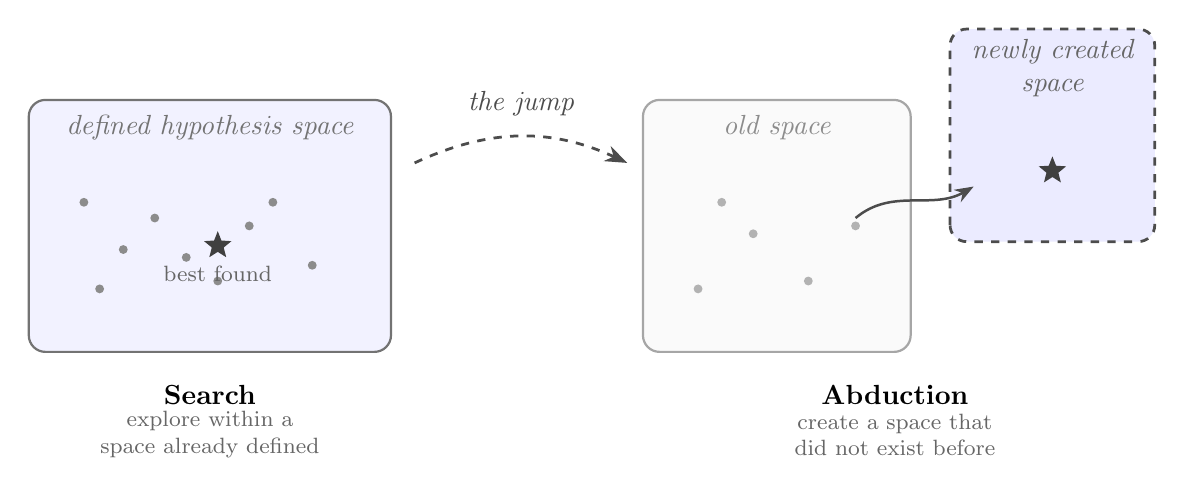
\begin{tikzpicture}[font=\small]
  \begin{scope}[shift={(0,0)}]
    \draw[rounded corners=6pt, draw=black!55, fill=blue!5, line width=0.8pt] (0,0) rectangle (4.6,3.2);
    \node[font=\itshape, text=black!55] at (2.3,2.85) {defined hypothesis space};
    \foreach \p in {(0.9,0.8),(1.6,1.7),(2.4,0.9),(3.1,1.9),(2.0,1.2),(3.6,1.1),(1.2,1.3),(2.8,1.6),(0.7,1.9)}
      \fill[black!45] \p circle (1.6pt);
    \node[star, star points=5, star point ratio=2.3, fill=black!75, inner sep=1.6pt] (best) at (2.4,1.35) {};
    \node[font=\footnotesize, text=black!60, below=0.5mm of best] {best found};
    \node[font=\bfseries] at (2.3,-0.55) {Search};
    \node[font=\footnotesize, text=black!60, align=center] at (2.3,-1.05) {explore within a\\ space already defined};
  \end{scope}
  \draw[-{Stealth[length=2.8mm]}, line width=1pt, draw=black!70, dashed] (4.9,2.4) to[out=25,in=155] (7.6,2.4);
  \node[font=\itshape, text=black!70] at (6.25,3.15) {the jump};
  \begin{scope}[shift={(7.8,0)}]
    \draw[rounded corners=6pt, draw=black!35, fill=black!2, line width=0.8pt] (0,0) rectangle (3.4,3.2);
    \node[font=\itshape, text=black!45] at (1.7,2.85) {old space};
    \foreach \p in {(0.7,0.8),(1.4,1.5),(2.1,0.9),(2.7,1.6),(1.0,1.9)} \fill[black!30] \p circle (1.6pt);
    \draw[rounded corners=6pt, draw=black!70, fill=blue!8, line width=1pt, dashed] (3.9,1.4) rectangle (6.5,4.1);
    \node[font=\itshape, text=black!60, align=center] at (5.2,3.6) {newly created\\ space};
    \node[star, star points=5, star point ratio=2.3, fill=black!75, inner sep=1.6pt] at (5.2,2.3) {};
    \draw[-{Stealth[length=2.4mm]}, line width=0.9pt, draw=black!70] (2.7,1.7) to[out=40,in=210] (4.2,2.1);
    \node[font=\bfseries] at (3.2,-0.55) {Abduction};
    \node[font=\footnotesize, text=black!60, align=center] at (3.2,-1.05) {create a space that\\ did not exist before};
  \end{scope}
\end{tikzpicture}
\caption{Search explores within a hypothesis space already defined. Abduction creates a space that
did not exist, the step an LLM has not been shown to take.}
\label{fig:jump}
\end{figure}

\subsection{Evidence on machine invention}
\label{sec:invention}

Two questions should be kept apart. The first is whether LLMs can produce outputs that people judge
novel. They can. In a controlled study with more than one hundred NLP researchers, Si, Yang, and
Hashimoto found that LLM-generated research ideas were rated more novel than those of human experts,
though less feasible~\cite{si2024}. Systems such as The AI Scientist automate much of the research
loop, generating ideas, writing and running code, and producing manuscripts, and report
experimentally evaluated contributions~\cite{aiscientist}. This is novelty of output.

The second question is whether an LLM has independently originated a new explanatory hypothesis whose
conceptual content was not already present in its training distribution, its prompt, its search
vocabulary, or a human-designed experimental frame. Here the evidence is thin. The reported novelty is
measured against a literature corpus or human judgment, and the autonomous systems run inside
substantial human scaffolding. An independent evaluation of The AI Scientist found that it often
labeled established techniques as novel and that many of its experiments and manuscripts were
flawed~\cite{aiscientisteval}. In a controlled molecular-genetics setting, Ding and Li report that a
generative model made incremental discoveries but not fundamental ones from scratch and did not
produce genuinely original hypotheses~\cite{dingli}. Zahavy frames the same gap as a missing abductive
step and takes Einstein's route to general relativity as the case~\cite{zahavy}.

The distinction is between novelty of output and novelty of hypothesis. The first is increasingly
demonstrated. The second remains open, and to our knowledge no published result has established it
with provenance showing the hypothesis was not inherited from the training data or the search frame.
LATSS does not settle the question. Section~\ref{sec:e12a} tests one part of it: when the predictive
feature is withheld from the vocabulary, more search does not recover it, because search cannot
recover information absent from the space it is given. An LLM may find a new solution inside a
financial hypothesis space without finding a new reason the market behaves as it does; the first is a
search problem, the second is the invention problem.

\subsection{Financial alpha}

Everything is decided before the search: which data is relevant, the prediction target, the horizon,
the available transformations, the evaluator, and the tests of success. A factor miner handed RSI,
volume, volatility, and momentum can find an expression nobody has written, and it remains a
construction from the given vocabulary. When the source of an anomaly is a variable that is not in
the vocabulary, not in the operator language, and not in the database, searching the given space
harder does not surface it, because the missing ingredient is outside the space. More compute, more
agents, deeper tree search, and a larger context window do not change this.

\subsection{Proposing hypotheses}

One response is to move the search up a level and ask the model for new variables and mechanisms,
which it supplies fluently: filing sentiment, supplier networks, options positioning. Each proposal
is an idea the model read somewhere, a recombination of hypotheses already written down. The proposed
variable is new to the reader, not to the world. Generating hypotheses is still search; the jump is
inventing one the space did not contain.

\subsection{Two ceilings}
\label{sec:two-ceilings}

Alpha resists automated discovery for two independent reasons. The cognitive ceiling is the inability
to produce a hypothesis outside $\mathcal{C}(D)$ (Section~\ref{sec:formal}), which is intrinsic to the
model. LeCun's critique that LLMs have no world model~\cite{lecun,lecunmtr} is a separate limitation
that scaffolding can lift: LATSS supplies a grounded world model externally, since the features are
measurements of the world and the backtest is the reality check, which is why the instrument of
Sections~\ref{sec:framework}--\ref{sec:results} works. Grounding tells the model whether a hypothesis
it already holds survives the data; it does not generate a hypothesis outside $\mathcal{C}(D)$. The
market-structure ceiling is that alpha is adversarial and perishable and its evaluator is causally
ambiguous: a successful backtest does not say why a factor predicted, whether mechanism, correlation,
hidden risk, regime, leakage, cost, or crowding. A new mechanism is necessary but not sufficient for
durable alpha, and the bar addresses overfitting within the search, not the missing hypothesis.

\subsection{Levels of novelty}
\label{sec:novelty}

Novelty covers four distinct achievements (Table~\ref{tab:novelty}), which lets a claim be held to a
matching standard of evidence. The first two can be reached by search within a supplied space; the
last two require evidence that the predictive premise was not already present in it.

\begin{table}[htbp]
\centering
\caption{Levels of novelty in automated alpha discovery. The last two require a hypothesis outside
the model's reachable set $\mathcal{C}(D)$.}
\label{tab:novelty}
\small
\begin{tabular}{@{}p{2.3cm} p{3.9cm} p{4.1cm} p{2.4cm}@{}}
\toprule
level & definition & evidence that would demonstrate it & state \\
\midrule
Syntactic & a formula no one has written & any run emitting a novel expression & routine \\[2pt]
Solution & a new construction for a defined problem & FunSearch cap-set and bounds~\cite{funsearch} & demonstrated \\[2pt]
Hypothesis & a new explanation for an unexplained phenomenon & a system originating a driver no source in $D$ contains, with a positive control & not demonstrated \\[2pt]
Economic & a new, durable, uncrowded source of returns & out-of-space edge surviving forward, after costs and crowding & none convincing \\
\bottomrule
\end{tabular}
\end{table}

The claim that current systems operate at the first two levels and have not reached the last two is
falsifiable. It is refuted by a system that, given raw data and no supplied vocabulary, repeatedly
originates durable, economically intelligible returns no source in its training data specified, with
a human or oracle positive control showing the step was achievable. We know of no such demonstration.
Reviewers rate LLM ideas as more novel than their own~\cite{si2024}, which measures how novel an idea
looks rather than whether it is real.

\subsection{Current systems}
\label{sec:audit}

Table~\ref{tab:audit} places representative systems by search space and novelty level. The level is a
qualitative classification we argue from each system's design, not a bibliographic fact. Each
recombines a human-defined primitive vocabulary, and we are aware of no published demonstration of one
originating an economic primitive no one specified. AlphaAgent's penalty on syntax-tree similarity to
crowded factors~\cite{alphaagent} is itself evidence that, unregularized, LLMs regenerate known
factors.

\begin{table}[htbp]
\centering
\caption{Representative LLM alpha systems by search space and novelty level (as in
Table~\ref{tab:novelty}); the level is a qualitative classification argued here.}
\label{tab:audit}
\small
\begin{tabular}{@{}p{3.3cm} p{5.3cm} p{2.1cm} p{1.4cm}@{}}
\toprule
system & primitive vocabulary / search space & machinery & level \\
\midrule
LATSS (this work) & given indicators to scoring rule & DE, null-max bar & 2 \\
AlphaAgent~\cite{alphaagent} & factor formulas over raw price/volume & multi-agent, AST penalty & 2 \\
Automate Strategy Finding~\cite{automate} & factor/strategy formulas over raw inputs & multi-agent, RL & 2 \\
CogAlpha~\cite{cogalpha} & factor formulas over raw inputs & LLM, tree search & 2 \\
QuantaAlpha~\cite{quantaalpha} & factor formulas over raw inputs & multi-agent & 2 \\
AlphaLogics~\cite{alphalogics} & logic and formula factors & search, verify & 2 \\
EFS~\cite{efs} & evolutionary factor formulas & evolutionary search & 2 \\
FunSearch~\cite{funsearch} (math) & programs for a defined problem & LLM, exact evaluator & 2 \\
\bottomrule
\end{tabular}
\end{table}

\subsection{Withholding the predictive feature (E12a)}
\label{sec:e12a}

The vocabulary boundary is measurable. We inject the signal into \code{feat\_c} as in
Section~\ref{sec:e1}, then overwrite the searcher's \code{feat\_c} with independent noise, so the
predictive feature is absent from the vocabulary. Across $\rho$ from 0 to 0.70, 30 seeds each, the
certification rate is zero at every signal strength, with the champion median near 0.43 against a bar
of 0.844. Section~\ref{sec:e1}, with \code{feat\_c} present, recovers reliably from $\rho=0.20$.
Recovery is governed by whether the predictive feature is in the vocabulary, not by signal strength
or search effort. We state the limit of this result directly: a mechanical searcher fails the same
way, so it demonstrates the vocabulary boundary and not an LLM-specific inability. A test that
isolates the LLM-specific step would need a semantically nameable driver together with a human or
oracle positive control, which the opaque synthetic driver here cannot provide, and we leave it to
future work.

\subsection{The ceiling}

The ceiling is the line between searching a hypothesis space and creating one, and current alpha
agents sit on the near side. LATSS is the alpha analogue of a coding agent: it generates, validates,
and recombines strategies from a human-supplied vocabulary under human supervision, scored against
the backtest much as a coding agent is scored against its tests. Both search and certify over known
primitives, and neither invents a new paradigm. Crossing the line would mean a system that, given raw
data and no predefined vocabulary, repeatedly finds durable, economically intelligible returns no one
told it to look for. We are aware of no such demonstration.

\section{Limitations}
\label{sec:limitations}

The validation uses one cross-validation scheme and the null-max bar as the gate, on a synthetic
cross-sectional oracle, which is a clean test of recovery rather than a model of how real alpha is
distributed. Certification is in sample against the bar by design, so the guarantee concerns the
strategy class's capacity to fit noise, not out-of-sample performance. The capacity result (E4) is
tested to ten thousand candidates and holds in part by construction; it does not rule out a loss of
power for a fixed weak signal at larger budgets, and the sign-flip null tests directional signal,
valid for this long-only task but not necessarily for a class with a non-directional overfitting
channel. The LLM comparison (E7) uses 3 seeds at three signal levels rather than a full LLM power
curve, and the search driver's per-run bar differs from the fixed mechanical bar, so we certify
against the fixed bar for comparability. The ceiling argument is reasoned rather than proved: a
universal negative is not provable, and the measurement in Section~\ref{sec:e12a} establishes the
vocabulary boundary rather than an LLM-specific failure to jump.

\section{Conclusion}

We presented LATSS and validated the loop as a measurement instrument rather than claiming a trading
strategy. On synthetic controls it rejects pure noise, with the certification frequency on noise
holding at 0 of 30 as the search budget grows to ten thousand candidates, recovers and certifies
injected signal from an active Sharpe near 0.66, and loses validity only under a mis-specified bar that
certifies noise in two of three runs. In a three-seed comparison the LLM-driven search recovers signal
at the same threshold as mechanical search, with no detectable advantage over the same vocabulary. We then examined the ceiling. LATSS, like other LLM
alpha-mining systems, searches a human-supplied hypothesis space rather than performing the abductive
step that creates a new one, and withholding the predictive feature drives recovery to zero at every
signal strength. External scaffolding can supply the grounded world model the LLM lacks; it cannot
supply the step that creates a new hypothesis space. Our experiments support treating an LLM-driven
loop as a measurement instrument for signal represented in its supplied vocabulary, rather than as
evidence that the loop originates new economic hypotheses.

\paragraph{Reproducibility.} The loop, the mechanical searchers, the skill bars, the
cross-validation, the synthetic test-bed, and the scripts producing every table are open source at
\url{https://github.com/vincent212/llm-assisted-trading-strategy-search}.

\begin{thebibliography}{99}

\bibitem{funsearch} B.~Romera-Paredes, M.~Barekatain, A.~Novikov, et al.
\newblock Mathematical discoveries from program search with large language models (FunSearch).
\newblock \emph{Nature}, 2023.

\bibitem{zahavy} T.~Zahavy.
\newblock LLMs Can't Jump (position paper). DeepMind, 2026.
\newblock \url{https://www.tomzahavy.com/projects/llms-cant-jump}.

\bibitem{si2024} C.~Si, D.~Yang, and T.~Hashimoto.
\newblock Can LLMs Generate Novel Research Ideas? A Large-Scale Human Study with 100+ NLP Researchers.
\newblock arXiv:2409.04109, 2024.

\bibitem{aiscientist} C.~Lu, C.~Lu, R.~T.~Lange, J.~Foerster, J.~Clune, and D.~Ha.
\newblock The AI Scientist: Towards Fully Automated Open-Ended Scientific Discovery.
\newblock arXiv:2408.06292, 2024.

\bibitem{aiscientisteval} J.~Beel, M.-Y.~Kan, and M.~Baumgart.
\newblock Evaluating Sakana's AI Scientist for Autonomous Research: Wishful Thinking or an Emerging
Reality?
\newblock arXiv:2502.14297, 2025.

\bibitem{dingli} A.~W.~Ding and S.~Li.
\newblock Generative AI lacks the human creativity to achieve scientific discovery from scratch.
\newblock \emph{Scientific Reports}, 2025. DOI 10.1038/s41598-025-93794-9.

\bibitem{lecun} R.~Balestriero, J.~Pesenti, and Y.~LeCun.
\newblock Learning in High Dimension Always Amounts to Extrapolation. arXiv:2110.09485, 2021.

\bibitem{lecunmtr} Y.~LeCun on world models. \emph{MIT Technology Review}, 2026.
\newblock \url{https://www.technologyreview.com/2026/01/22/1131661/yann-lecuns-new-venture-ami-labs/}.

\bibitem{deprado} M.~L\'opez de Prado.
\newblock \emph{Advances in Financial Machine Learning}. Wiley, 2018.

\bibitem{deflated} D.~H.~Bailey and M.~L\'opez de Prado.
\newblock The Deflated Sharpe Ratio. \emph{Journal of Portfolio Management}, 2014.

\bibitem{nullmax} V.~Maciejewski.
\newblock What Is the Null-Max Bar, and Could It Replace the Deflated Sharpe Ratio? 2026.
\newblock \url{https://vincentmayeski.substack.com/p/what-is-the-null-max-bar-and-could}.

\bibitem{vapnik} V.~N.~Vapnik. \emph{Statistical Learning Theory}. Wiley, 1998.

\bibitem{bartlett} P.~L.~Bartlett and S.~Mendelson.
\newblock Rademacher and Gaussian Complexities. \emph{JMLR}, 3:463--482, 2002.

\bibitem{alphaagent} AlphaAgent: LLM-Driven Alpha Mining with Regularized Exploration to Counteract
Alpha Decay.
\newblock arXiv:2502.16789, 2025.

\bibitem{automate} Z.~Kou, H.~Yu, J.~Luo, et al.
\newblock Automate Strategy Finding with LLM in Quant Investment.
\newblock arXiv:2409.06289, 2024 (Findings of EMNLP 2025).

\bibitem{cogalpha} F.~Liu et al.
\newblock Cognitive Alpha Mining via LLM-Driven Code-Based Evolution.
\newblock arXiv:2511.18850, 2025.

\bibitem{hubble} Celestial Quant Lab.
\newblock Hubble: An LLM-Driven Agentic Framework for Safe, Diverse, and Reproducible Alpha Factor
Discovery.
\newblock arXiv:2604.09601, 2026.

\bibitem{quantaalpha} J.~Han et al.
\newblock QuantaAlpha: An Evolutionary Framework for LLM-Driven Alpha Mining.
\newblock arXiv:2602.07085, 2026.

\bibitem{alphalogics} Z.~Weng, S.~Zhang, T.~Wang, and Y.~Xia.
\newblock AlphaLogics: A Market Logic-Driven Multi-Agent System for Scalable and Interpretable Alpha
Factor Generation.
\newblock arXiv:2603.20247, 2026.

\bibitem{efs} H.~Luo, Y.~Zhang, and C.~Liu.
\newblock EFS: Evolutionary Factor Searching for Sparse Portfolio Optimization Using Large Language
Models.
\newblock arXiv:2507.17211, 2025.

\bibitem{evolutionalpha} M.~R.~Islam.
\newblock The Evolution of Alpha in Finance: Harnessing Human Insight and LLM Agents.
\newblock arXiv:2505.14727, 2025.

\end{thebibliography}

\end{document}
